\documentclass{article}

\usepackage{caption}
\usepackage{enumitem}
\usepackage{graphicx}
\usepackage{float}
\usepackage{amssymb}

\usepackage[
	backend=bibtex
]{biblatex}
\addbibresource{refs.bib}
\captionsetup{
	labelfont=bf,
	font=small,
	justification=centering
}
\renewcommand{\figurename}{Fig.}

\usepackage[
	hypertexnames=false,
	colorlinks=true,
	citecolor=blue
]{hyperref}

\title{
	Canning for Amorphous Blob Computing\\
	\small TER report
}

\author{
    Auteur :\\
    Lucas Labouret\\
    M1 QDCS, Université Paris-Saclay\\
    \small lucas.labouret@universite-paris-saclay.fr
    \and
    Encadrant :\\
    Frédéric Gruau\\
    LISN\\
    \small frederic.gruau@universite-paris-saclay.fr
}

\date{}

\begin{document}
 
\maketitle

\begin{figure}[H]
	\centering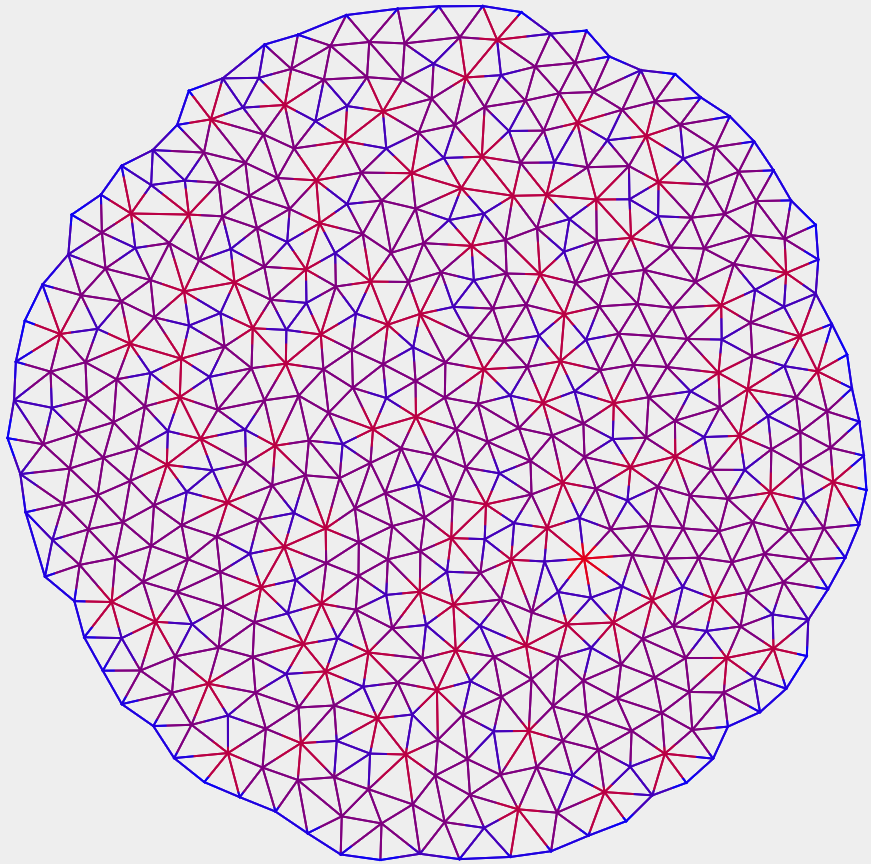
\includegraphics[width=0.9\linewidth]{assets/Circle500.png}
\end{figure}

\newpage
\tableofcontents
\newpage

\renewcommand{\thesection}{\Alph{section}}

\section{What is Blob Computing ?}

This TER is part of a long term research project about the concept of "blob computing"\supercite{blob_computing1}. To understand the exact subject of this TER, it is important to first introduce what blob computing means and how it works.\\

The ultimate goal of the project is to develop a new paradigm of computation that is inherently arbitrarily scalable through the use of \textit{space} as a resource. This kind of computation is becoming increasingly useful, for example with the recent development of swarm robotic\supercite{swarm_robotic}.

We aim to achieve this through the use of arbitrarily many processing elements (PEs) distributed through space and locally connected. These PEs, which can be severely lacking in power on their own, create a computing medium where virtual "blobs" can form and evolve. These blobs are the main primitive we use for making computations. 

IMPORTANT $\longrightarrow$ blobs persist through time

\subsection{Definition and Structure of a Computing Medium}

\begin{figure}[H]
	\centering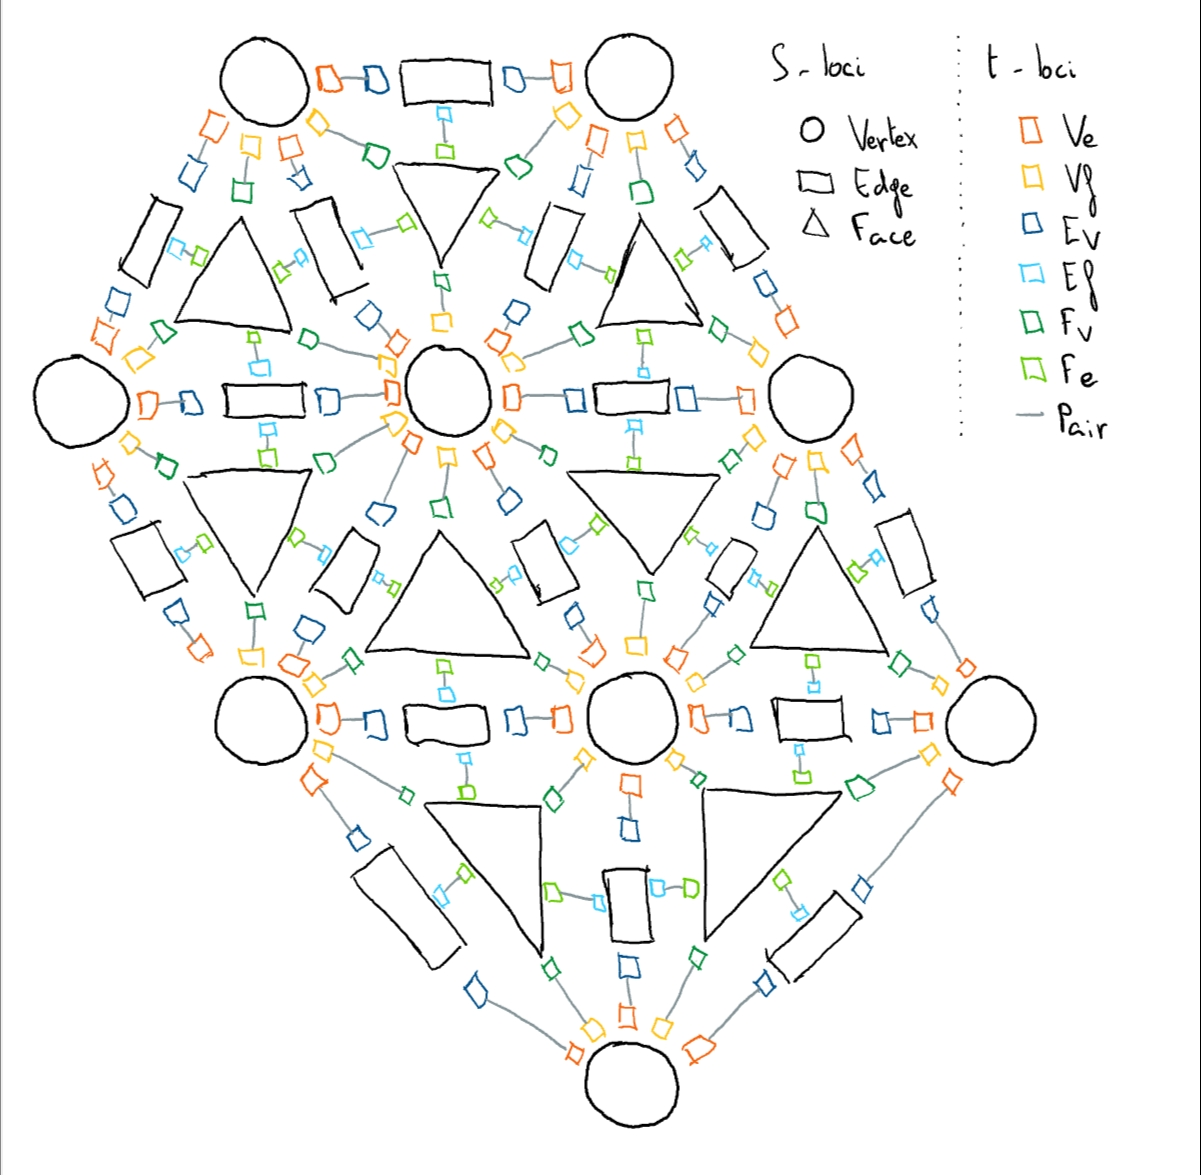
\includegraphics[width=0.9\linewidth]{assets/handdrawn_medium.png}
	\caption{Example structure of a medium.}
	\label{fig:example_structure}
\end{figure}

In general, a computing medium graph where each vertex, edge, and face is associated with a processing element capable of executing minimal computation, storing information, and communicating with its neighbors. Here, we focus exclusively in specific mediums which are weakly Delaunay triangulated, hence the term "computing medium" in the rest of this report will refer to those unless specified otherwise.

Vertices, edges and faces are called "simplicial loci" (or "S-loci" for short). They determine the overall structure of their medium. Each S-locus controls a set of "transfer loci" (or "t-loci"). T-loci come in pairs that handle the communication between two S-loci. For example, if a vertex was connected to an edge, there would be a pair of t-loci (one belonging to the vertex and the other belonging to the edge) between them.

Obviously, there are 3 types of S-loci : Vertex, Edge, Face. T-loci are divided into 6 types : 
\begin{itemize}[noitemsep,nosep]
	\item Ve linking a  Vertex to an Edge
	\item Vf linking a  Vertex to a  Face
	\item Ev linking an Edge   to a  Vertex
	\item Ef linking an Edge   to a  Face
	\item Fv linking a  Face   to a  Vertex
	\item Fe linking a  Face   to an Edge
\end{itemize}
Figure~\ref{fig:example_structure} show an example of how all these loci are put together to form a medium.

A medium is said to be crystalline if a repeating structure emerges in the placement if its vertices. It is amorphous when no such structure emerges. Additionally, it is homogeneous if the average point density is approximately constant and there are no
“holes” or “clusters”, and it is isotropic if the directions of the edges of the medium follow a uniform distribution over $[0, \pi[$. This report mainly focuses on amorphous homogeneous isotropic (AHI) media.

\begin{figure}[H]
	\centering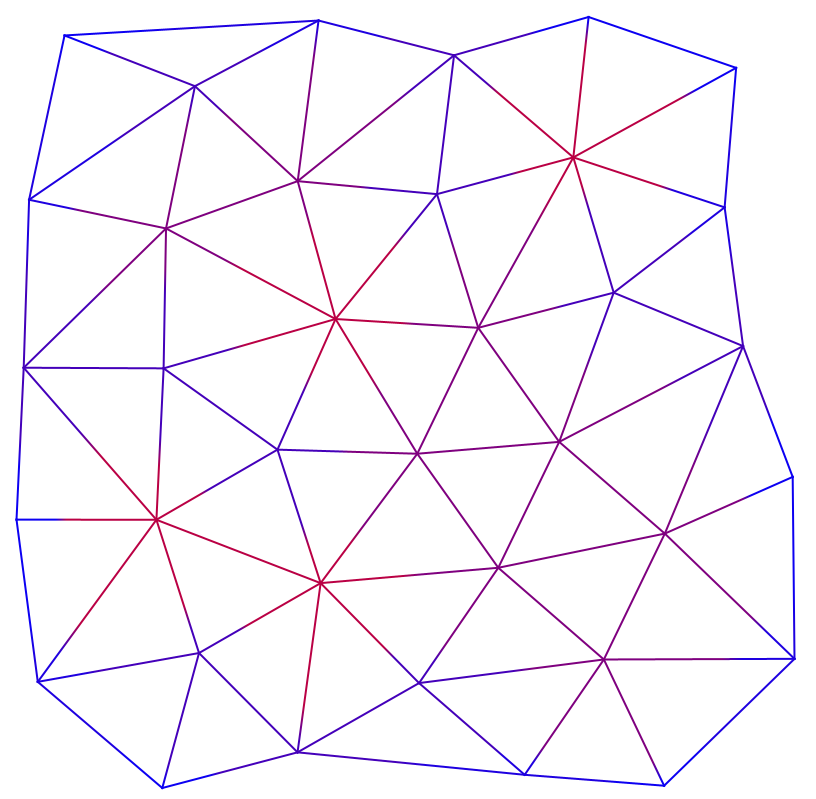
\includegraphics[width=0.4\linewidth]{assets/amorphous_medium.png}
	\hspace{0.1\linewidth}
	\centering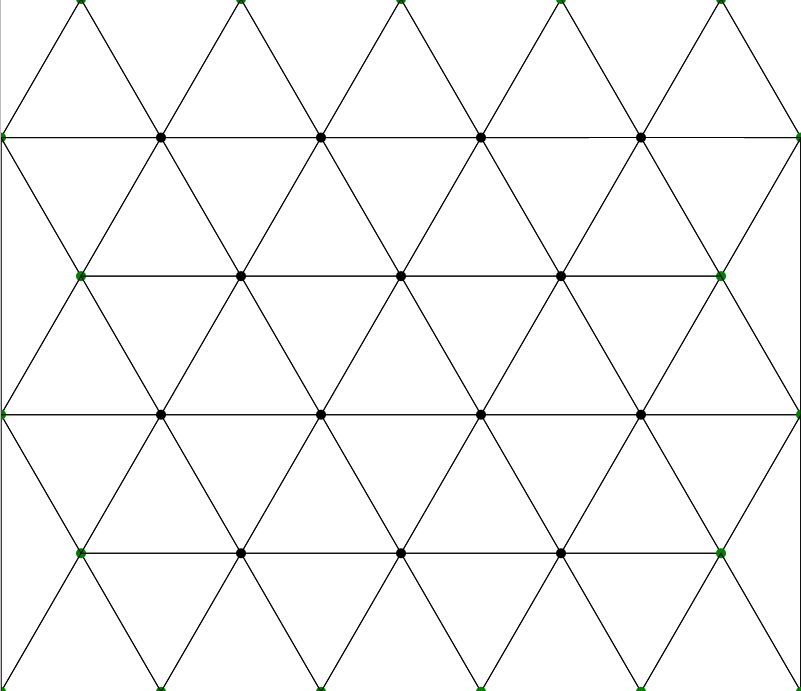
\includegraphics[width=0.4\linewidth]{assets/hexagonal_medium.png}
	\caption{An AHI medium (left) VS a crystalline hexagonal medium (right).}
	\label{fig:amorphous_vs_crystaline}
\end{figure}

For now, we consider PEs to be immobile and synchronous, although lifting these two constraints will probably be the subject of future research.\\

A blob of a given medium $M$ is a connected sub-graph $M'$ of $M$ such that all the vertices of $M'$ share a common property (e.g.: all their values are even, or all their values are 1, etc.). Depending on the program, these blobs are able to grow, shrink, merge, divide and more, which is the computational basis of blob computing\supercite{blob_computing2}.

\subsection{An Example of Computation : the Voronoï Diagram}

\cite{Voronoi} develops tools to program on computing media. As an example, it shows how to build a (discrete) Voronoï diagram from a set of "seeds" in a medium.

\begin{figure}[H]
	\centering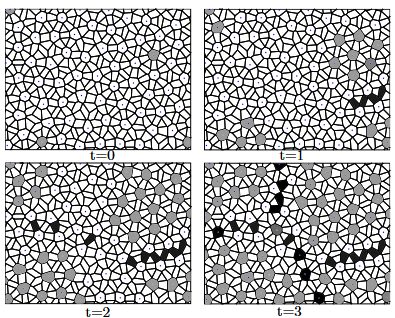
\includegraphics[width=0.7\linewidth]{assets/voronoi_spread.png}
	\caption{
		Computation of a discrete Voronoï diagram.\\
		Cells marked with a dot are the vertices of the medium.
		Gray cells form blobs. Black cells mark the frontiers between blobs. At t=0, blobs only cover the seeds. At t=3, blobs cover the Voronoï regions of the medium.\\
		\textit{Source : \cite{Voronoi}}
	}
	\label{fig:voronoi_spread}
\end{figure}

The basic idea is the following : we start with a set of "seeds" distributed over the vertices of the network. Each seed is now the center of a blob. Then, at each synchronous step, the blobs will spread to their adjacent vertices if this wouldn't cause them to merge with another blob, until no blob can spread further. It can be implemented with very few types of local operations that are applied simultaneously to every S-locus in the network :
\begin{itemize}
	\item Multi-cast\\
	The S-locus copies its value into its t-loci of a given type.
	\item Rotation\\
	Since t-loci are spatially arranged around their S-loci, we can define a clockwise and counter-clockwise neighbor. T-loci can perform logical operations on their and their neighbors' values.
	\item Reduction\\
	The S-locus stores the result of a commutative and associative operation applied to the values of its t-loci of a given type.
	\item Transfer\\
	Each of the S-locus' t-loci exchanges its value with the value of its pair. 
\end{itemize}
In fact, clever association of these primitives allows to program everything a computing medium is capable of, such as sorting arrays of integer or multiplying matrices\supercite{blob_computing2}.

\subsection{Objective : Cannings}

Up until now, Gruau mainly focused on hexagonal crystalline media. He built a plateform allowing efficient simulation of blob computation on classical hardware using SIMD\supercite{Voronoi, platform_CA2}. 

The point of this TER is to allow the use of SIMD to optimize the simulation of AHI media as well. We do this through the development of the notion of "total canning", or simply "canning". Given a medium $M$, a canning is a set of 9 injective maps which assign some integer coordinates to each locus of $M$ :
\begin{enumerate}[noitemsep,nosep]
	\item $\{$Vertex$_M\} \mapsto \mathbb{N}^{a_1}$
	\item $\{$Edge$_M\} \mapsto \mathbb{N}^{a_2}$
	\item $\{$Face$_M\} \mapsto \mathbb{N}^{a_3}$
	\item $\{$Ve$_M\} \mapsto \mathbb{N}^{a_4}$
	\item $\{$Vf$_M\} \mapsto \mathbb{N}^{a_5}$
	\item $\{$Ev$_M\} \mapsto \mathbb{N}^{a_6}$
	\item $\{$Ef$_M\} \mapsto \mathbb{N}^{a_7}$
	\item $\{$Fv$_M\} \mapsto \mathbb{N}^{a_8}$
	\item $\{$Fe$_M\} \mapsto \mathbb{N}^{a_9}$
	\item[] where $a_1, ..., a_9 \geq 1$ are specific to each canning method.
\end{enumerate}
Through misuse of language, the term "canning" will designate either this set of maps, or the algorithm used to build it.

The objective is twofold : firstly, we want to find a way to measure the efficiency of a canning on a given medium. Secondly, we want to create a canning that is efficient on most -if not all- media.

\section{Preliminary Work}

In this section, I briefly introduce some work I did last year during another internship with Gruau to generate AHI media. While it isn't the main focus of this year's interniship, it is what made it possible in its current form.

\subsection{Delaunay Triangulation}

A Delaunay triangulation is a particular type of triangulation where a triplet of vertices form a face iif no other vertex can be found inside the circumcircle of the triplet. We relax this definition slightly by allowing the hull of the graph not to be convex. It presents interested properties for our purpose as the edges of the triangulation tend to remain "localized" (i.e. vertices that are connected tend to be spatially close).

I used the triangulation algorithm described in \cite{build_delaunay}. However, there is a bug in my implementation where vertically-aligned are often handled incorrectly, which I couldn't fix before the end of my internship last year. Since this problem wasn't particularly consequential this year either, I didn't take the time to fix it this year either.

Additionally, the FPO algorithm (see \ref{fpo}) performs a lot of removals and insertions to the set of vertices. Currently, each time this happens, the entire set is retriangulated. This is a vastly inefficient approach to the problem. If I had the time, I would've liked to implement the removal and addition algorithms described in \cite{build_delaunay, remove_delaunay}.

\subsection{Farthest Point Optimization}
\label{fpo}

The Farthest Point Optimization algorithm \supercite{FPO} allows the construction of the irregular yet homogeneous sets of points that we need for blob computing. It yields better results than more common algorithm like Poisson-Disk sampling or Lloyd algorithm, and fits naturally into the project as it relies heavily on the Delaunay triangulation.

The implementation of FPO in my case wasn't straightforward. This is because the article applied the algorithm to sets of points in the unit torus, while the media use bounded subsets of the euclidean plane instead. In particular, I had to adapt the algorithm to work around the existence of borders with no predetermined shape, and that can contain fixed points that cannot be moved even though they can still influence the placement of other points.

\renewcommand{\thesection}{\arabic{section}}
\setcounter{section}{0}

\section{Borders and Media}

\subsection{Choice of Border}

\subsection{Different Types of Medium}

\section{Canning and Evaluation}

Before we begin our search for total cannings, let us define the notion of partial canning. A partial canning of a medium $M$ is simply a subset of a total canning of $M$ (or the algorithm used to build it). In particular, we focus on vertex cannings, i.e. partial cannings which only contain the map from the vertices of $M$ to their coordinates. From there, we will exhibit a generic method for build total cannings using vertex canning as a base. Finally, we will show how we can evaluate the efficiency of different cannings so we can compare them.

\subsection{Vertex Cannings}
\label{partial_canning}

For now, we set $a_1$ (the n), the objective is equivalent to placing every vertex of the medium in a grid s.t. every cell of the grid contains at most 1 vertex. For now, I explored two vertex cannings with opposed philosophies :
\begin{enumerate}
	\item \textbf{TopDistanceXStorted} vertex canning\\
	This vertex canning was developed to rely as much as possible on the graph structure of the medium, making as little use as possible of its spatial aspect. It was developed quite early in the project, before soft-bordered media appeared, so it only works on hard-bordered media. It works in the following way :\\
	- First, compute the minimum graph-distance of each vertex to any vertex on the topside of the border. All vertices at distance Y from the top are placed in line Y of the grid.\\
	- Second, place the leftmost vertex of each line in the first cell of its line, the second leftmost vertex of each line in the second cell of its line, repeating until all vertices are placed in the grid.
	
	\item \textbf{RoundedCoordinates} vertex canning\\
	This vertex canning was developed to rely exclusively on the spatial embedding of the medium, completing ignoring its graph structure. It works in the following way :\\
	- First set a counter to 1.\\
	- Multiply the spatial coordinates of each vertex by the counter and round the result. Use the two integers obtained as a 2D index to put each vertex in the grid.\\
	- If two vertices share the same cell, increment the counter by one and go back to the previous step. Otherwise, we have a vertex canning.
\end{enumerate}

\begin{figure}[H]
	\centering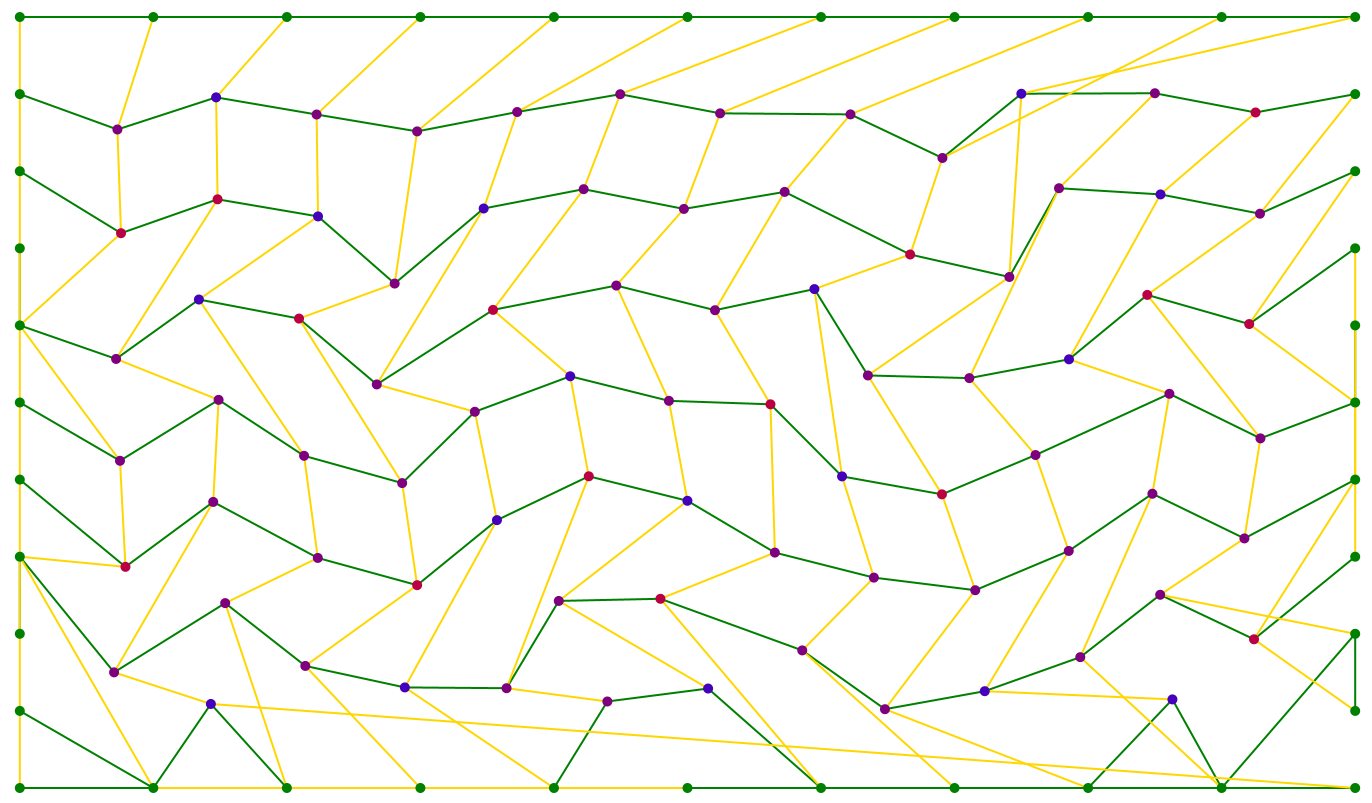
\includegraphics[width=0.45\linewidth]{assets/TopDistanceXSorted.png}
	\centering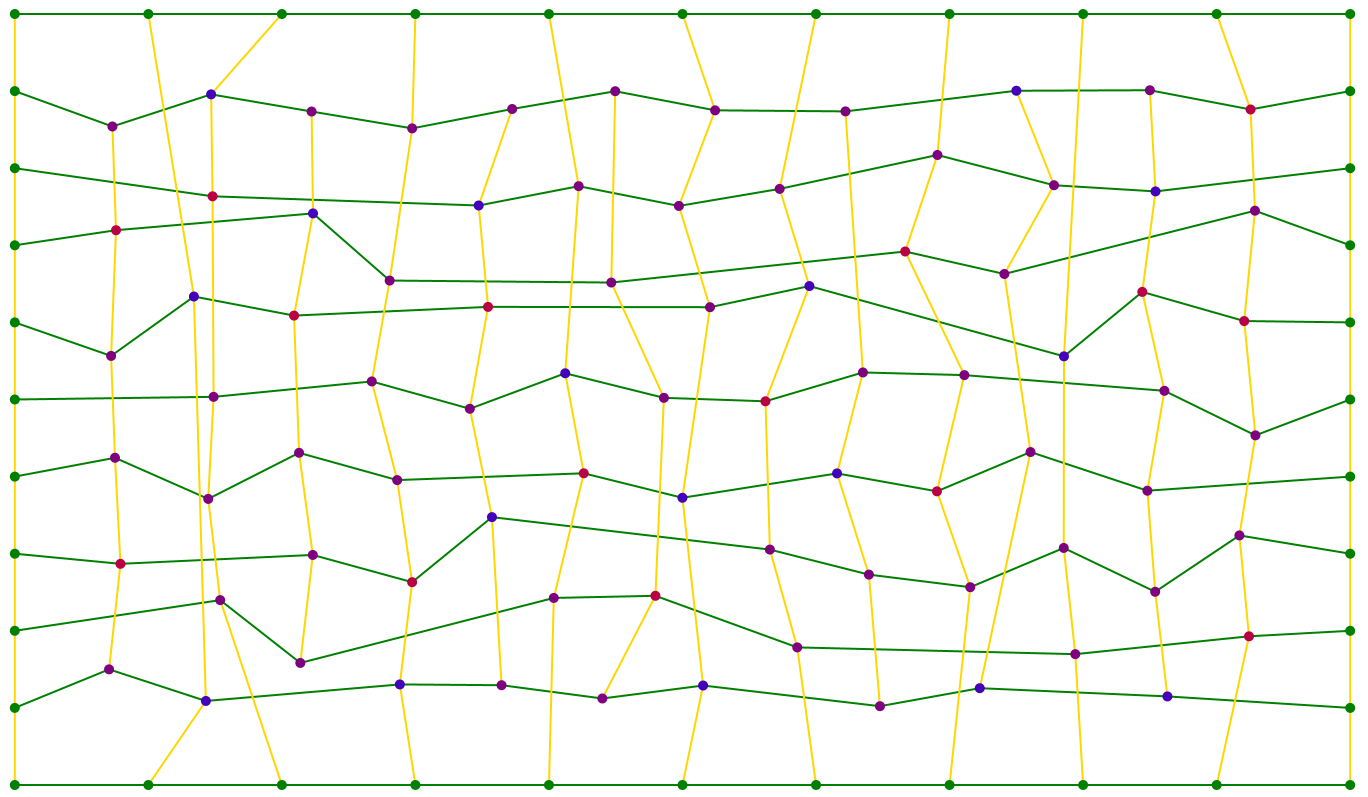
\includegraphics[width=0.45\linewidth]{assets/RoundedCoordinates.png}
	\caption{TopDistanceXSorted (left) next to RoundedCoordinates (right) applied to the same medium.\\
	Two vertices are joint by a green line if they are consecutive on a line of the grid, and a yellow line if they are consecutive in a column.}
	\label{fig:topdist_vs_rounded}
\end{figure}

\subsection{From Vertex to Total Cannings}



\subsection{Evaluation}

\section{GUI}

A large portion of the TER was focused on the development of a software equipped with a GUI that allows the user to
\begin{enumerate}[noitemsep,nosep]
	\item Randomly generate new media, save them, and load them.
	\item Visualize different aspects of the media.
	\item Compute and visualize different cannings.
\end{enumerate}
$ $

If developing a GUI for this application ended up being time-consuming, it was incredibly helpful all around while debugging everything else. Overall it was probably a net positive on development time alone, and that is still neglecting the advantage of being able to see what i am doing.\\
$ $

Below are some pictures of the kind of visualization the GUI provides.

\begin{figure}[H]
	\centering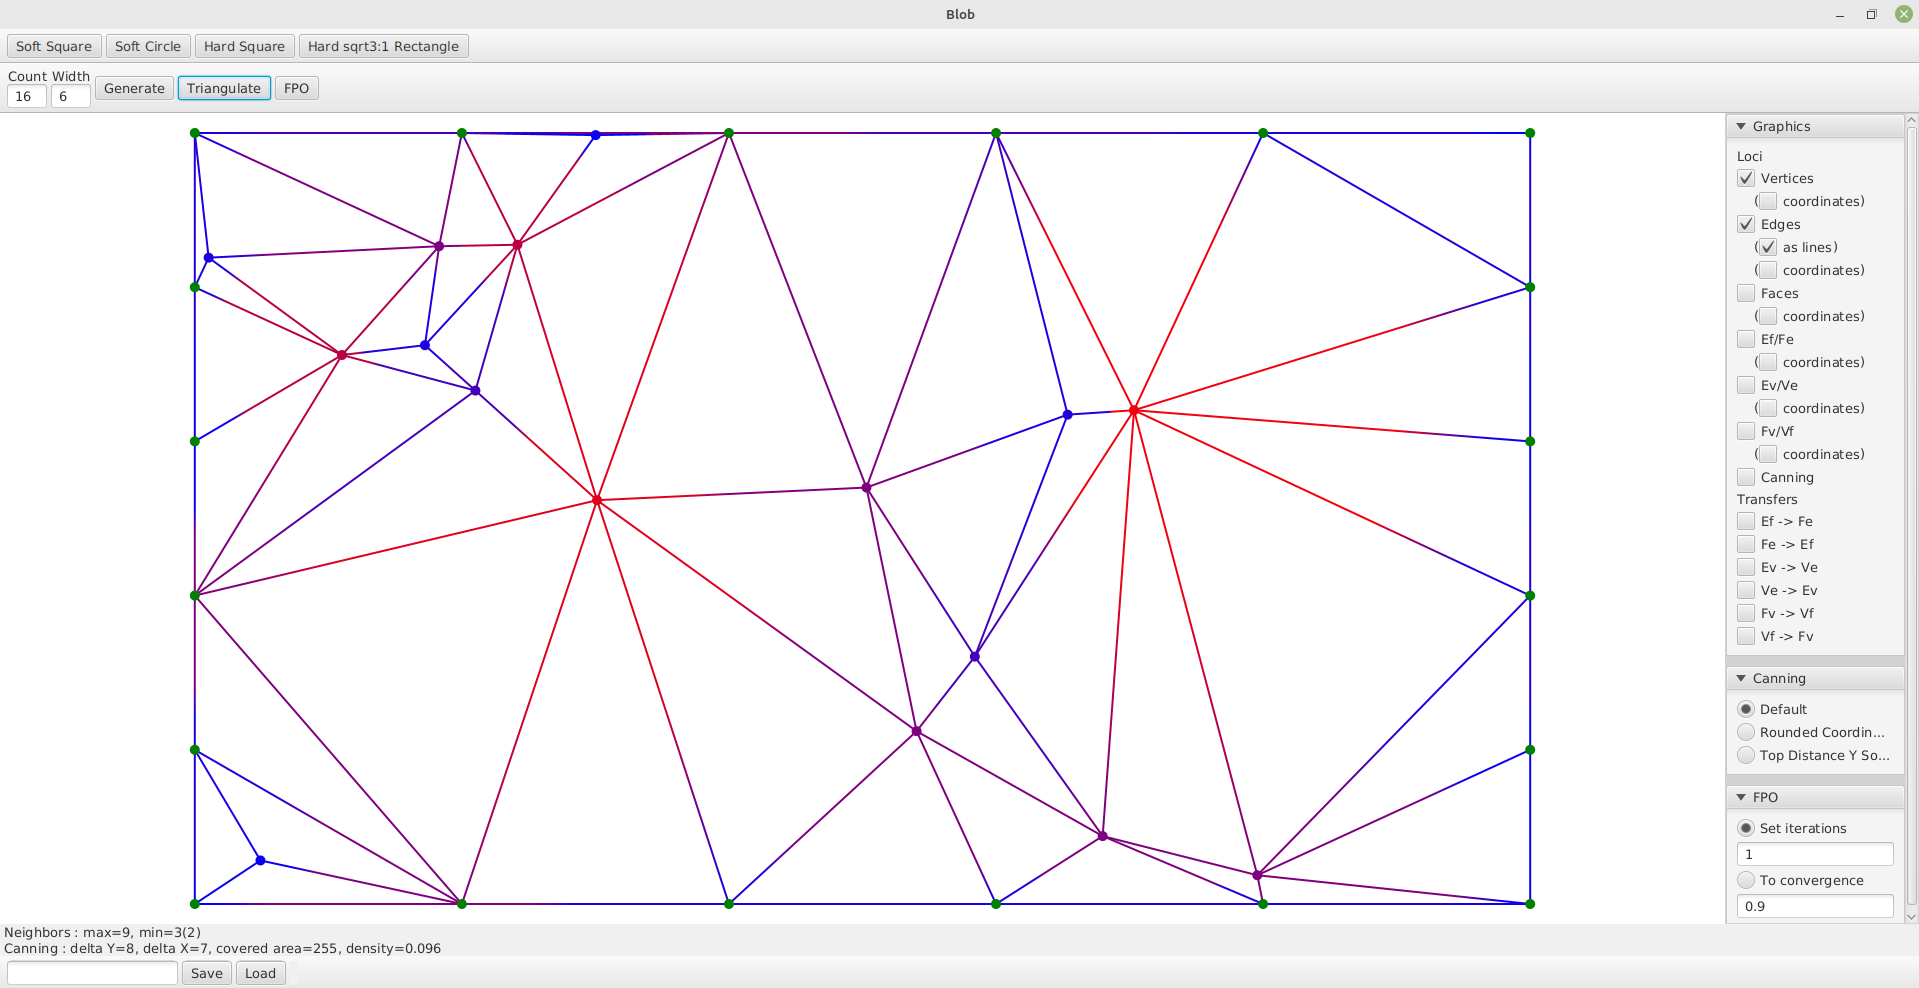
\includegraphics[width=0.8\linewidth]{assets/canonical_before.png}
	\centering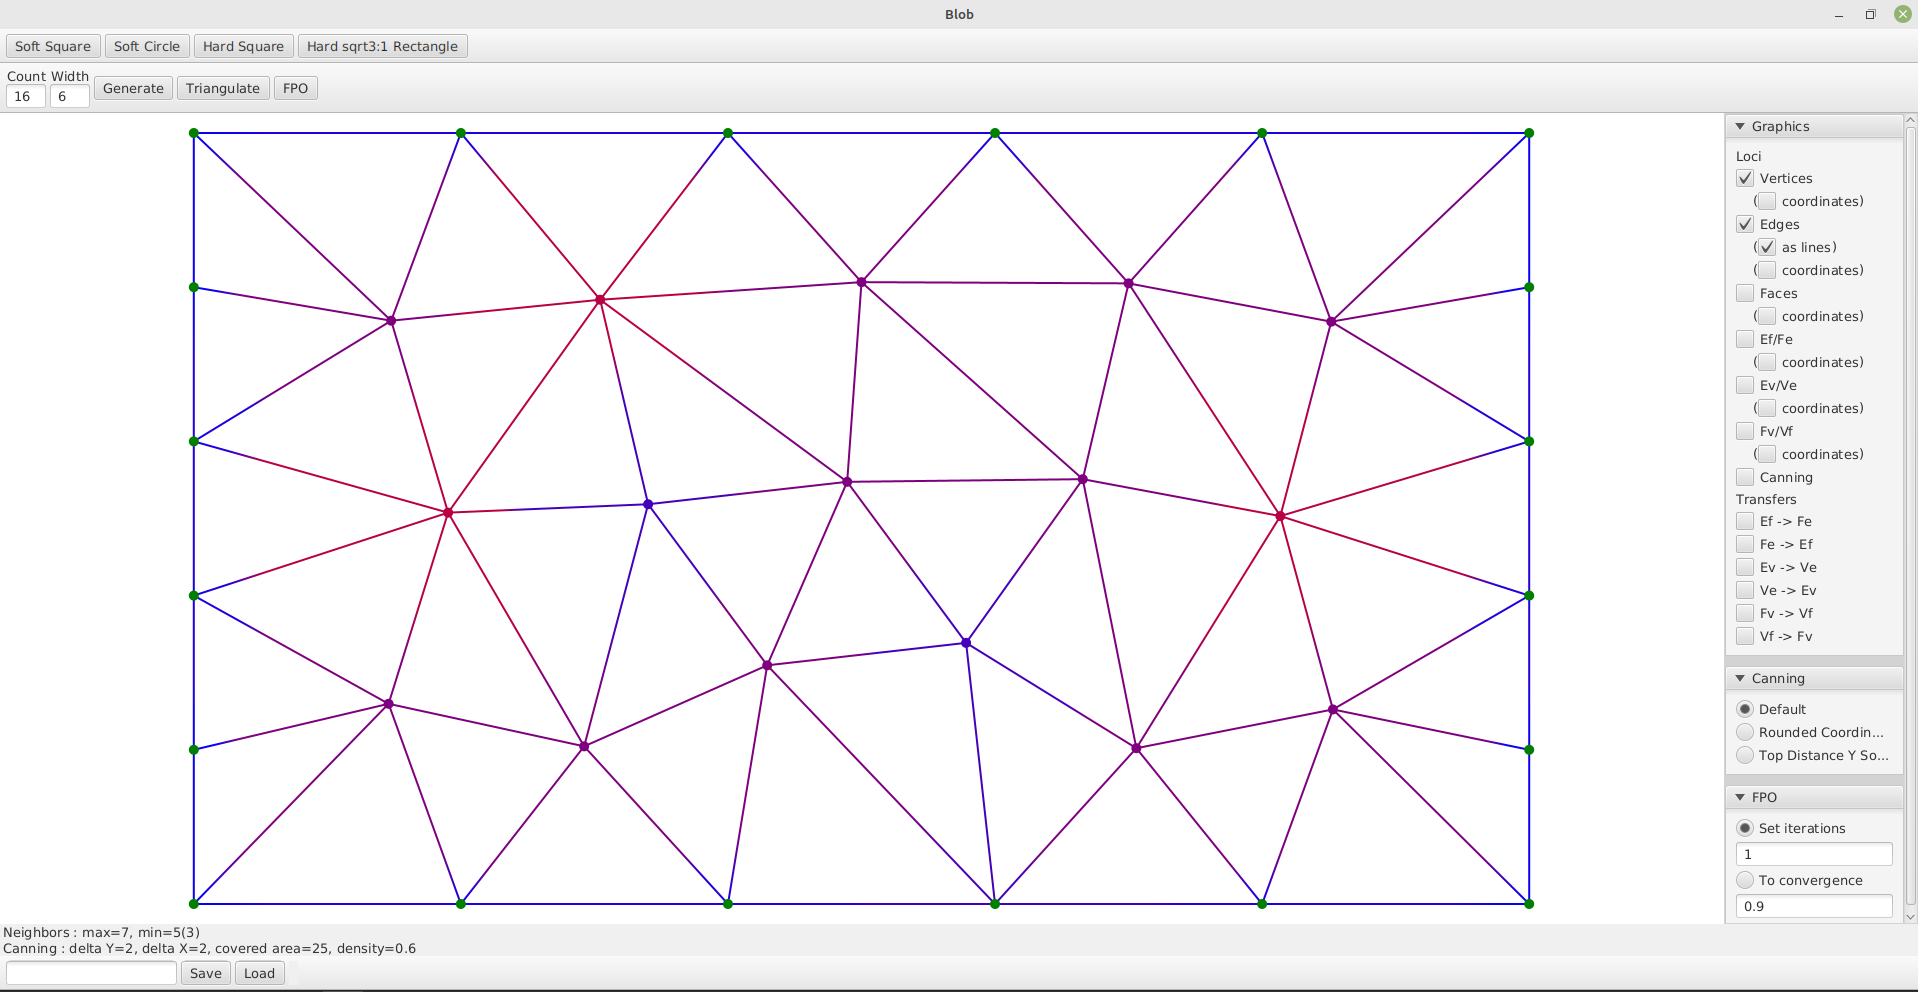
\includegraphics[width=0.8\linewidth]{assets/canonical_after.png}
	\caption{"Canonical" view of a medium before (top) and after (bottom) optimization with FPO.}
	\label{fig:gui_before_after_FPO}
\end{figure}

\begin{figure}[H]
	\centering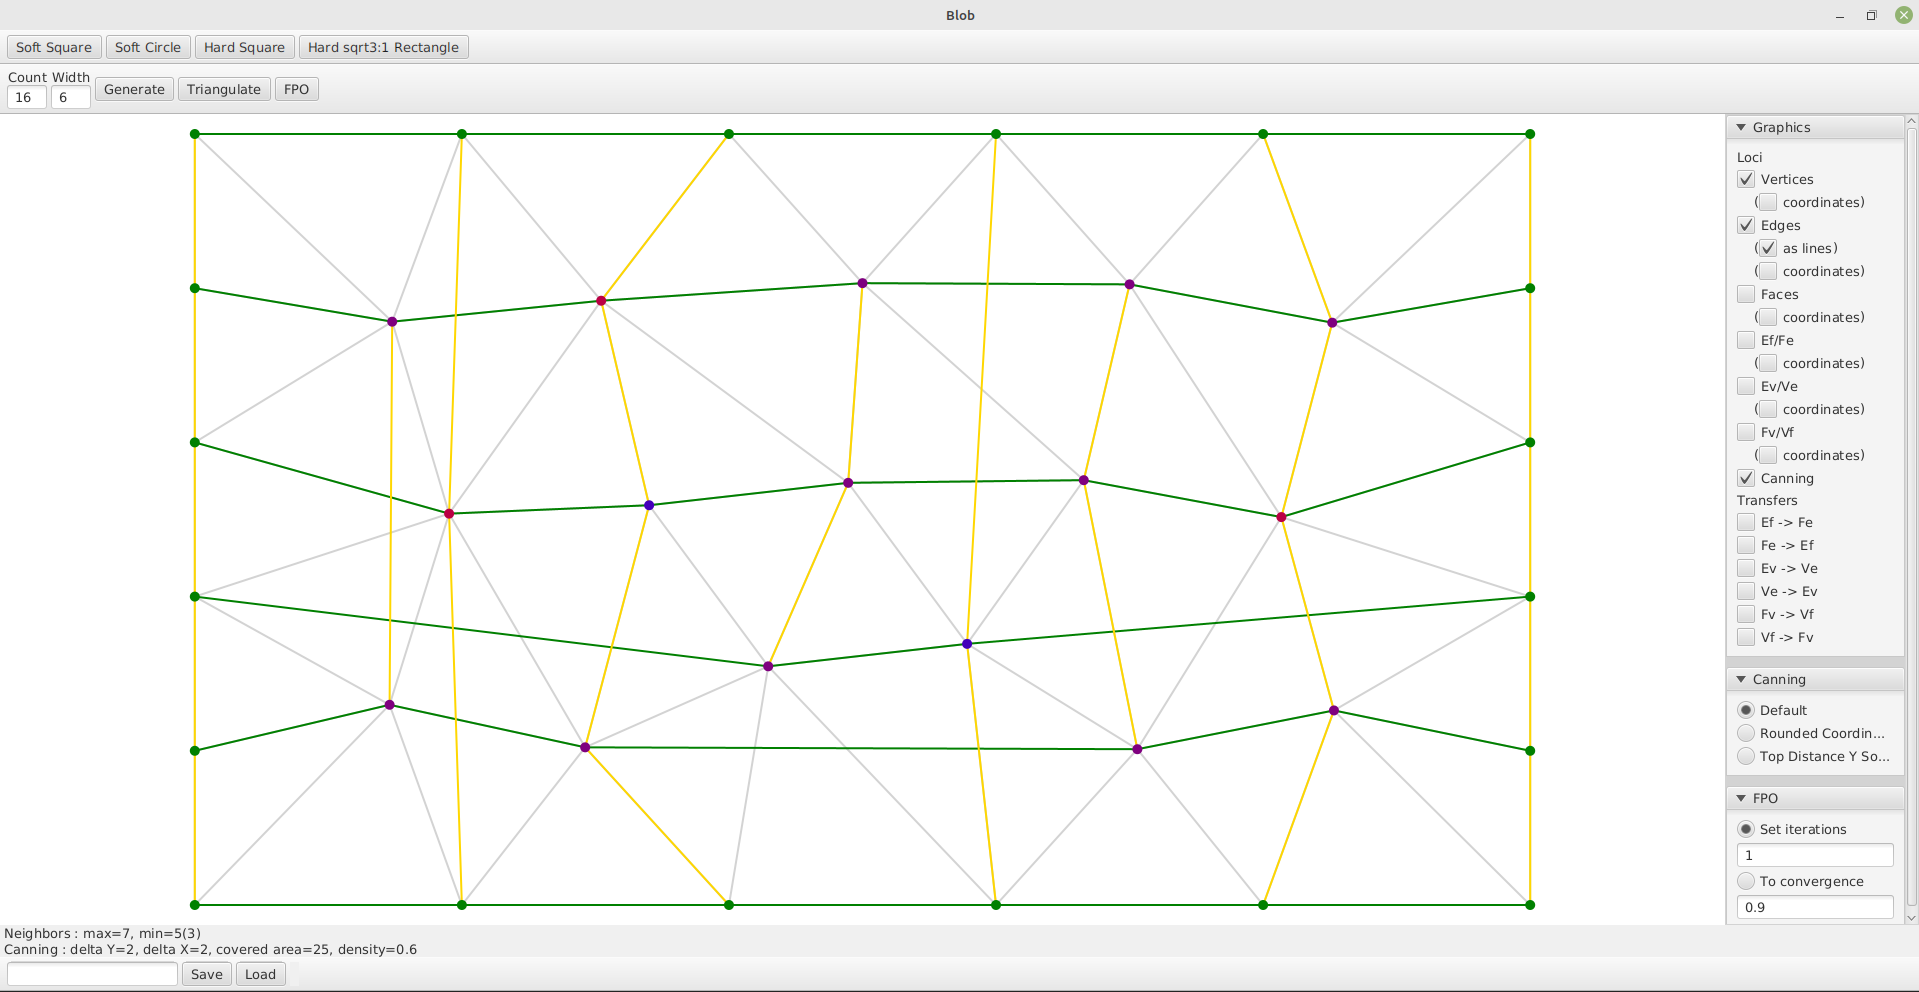
\includegraphics[width=0.8\linewidth]{assets/canning_view.png}
	\caption{View of a partial canning (see \ref{partial_canning}) of the vertices of the medium in figure~\ref{fig:gui_before_after_FPO}}
	\label{fig:gui_canning}
\end{figure}

\begin{figure}[H]
	\centering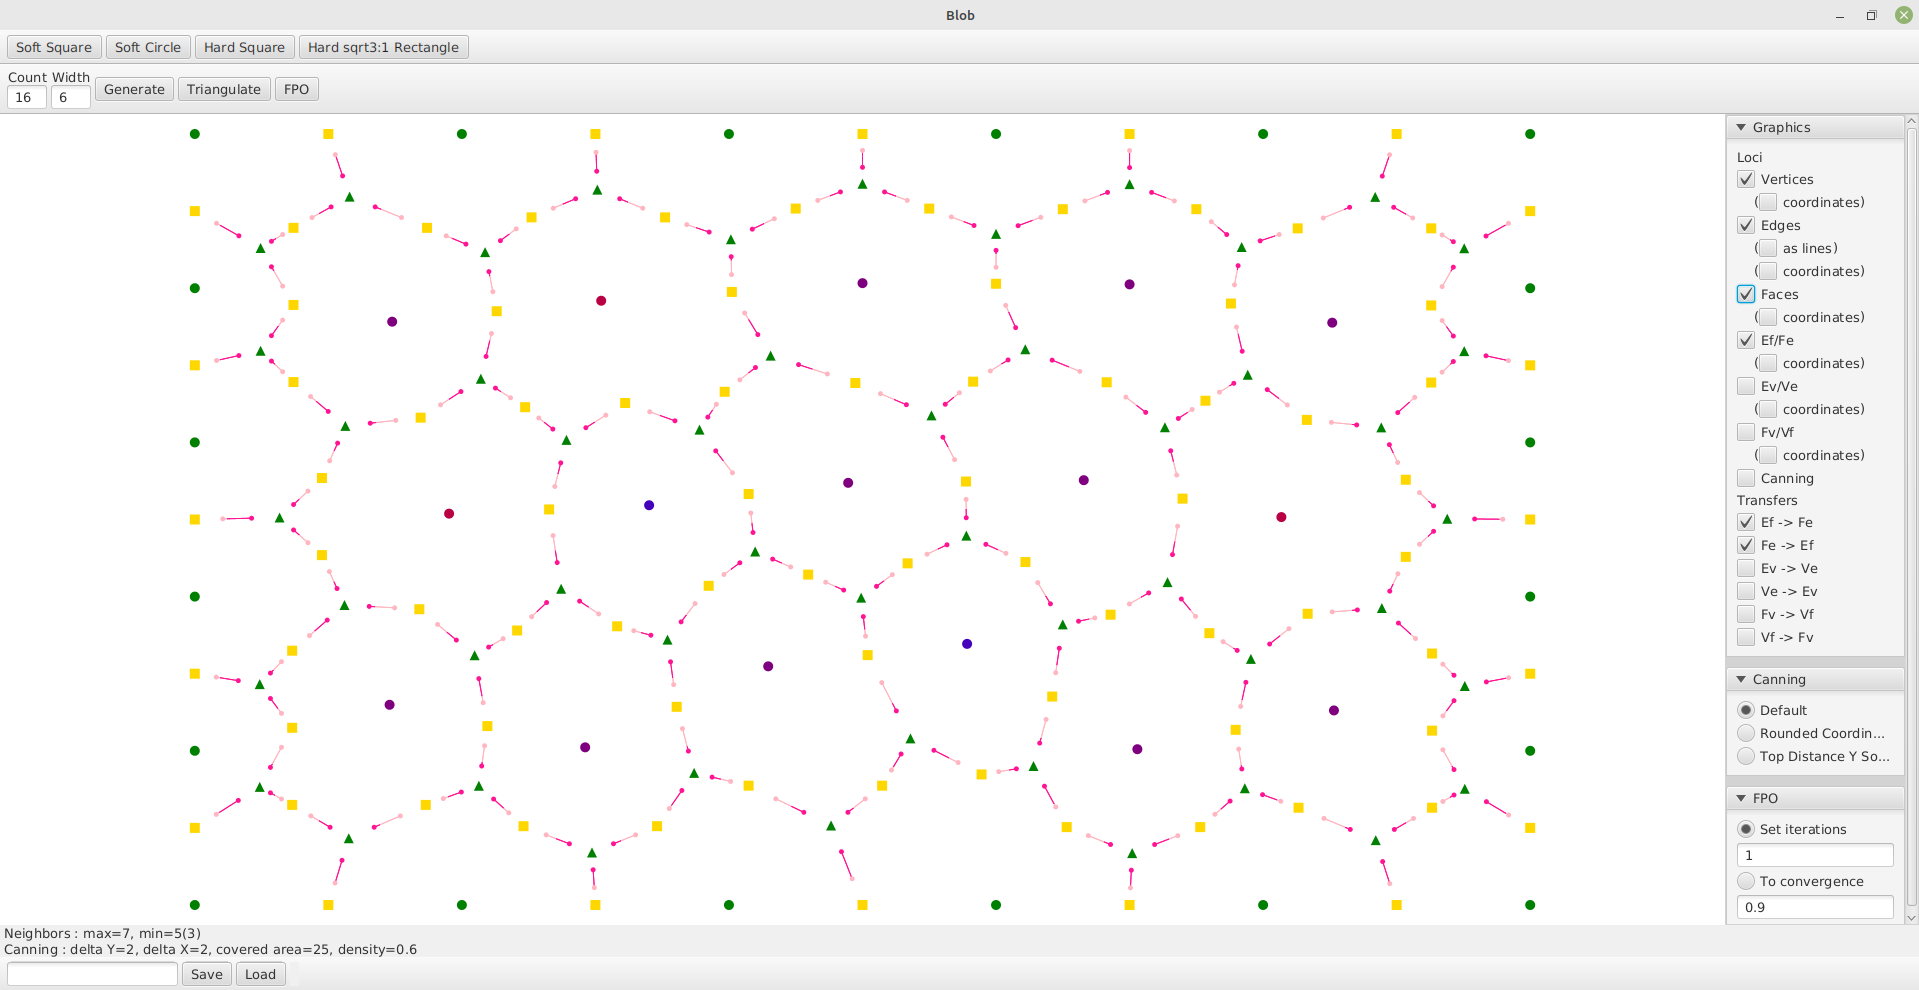
\includegraphics[width=0.8\linewidth]{assets/EfFe_transfers.png}
	\caption{View of the Ef-Fe pairs in the medium of figure~\ref{fig:gui_before_after_FPO}.}
	\label{fig:gui_EfFe}
\end{figure}

\section{Conclusion}

\printbibliography[heading=bibintoc]

\end{document}
